%!TEX root = ../main.tex
\chapter{Miniproject 2}
\section{XQuery}

Since we are using Express, we made the XQuery exercise in our web app. We also used a tool called BaseX as an XQuery server.

We used the data file from \url{http://www.cs.washington.edu/research/xmldatasets/data/courses/uwm.xml}.
It contains university courses, and related information.

The XML data we used as input was as the format in \cref{lst:xmldataexample}.

\begin{listing}
    \begin{xmlblock}
        <?xml version="1.0" encoding="UTF-8"?>
        <root>
            <course_listing>
                <note>#</note>
                <course>216-293</course>
                <title>BUSINESS ETHICS</title>
                <credits>3</credits>
                <level>U</level>
                <restrictions>; ; PREREQ: NONE</restrictions>
                <section_listing>
                    <section_note/>
                    <section>Se 001</section>
                    <days>R</days>
                    <hours>
                        <start>2:30pm</start>
                        <end>5:10pm</end>
                    </hours>
                    <bldg_and_rm>
                    <bldg>BUS</bldg>
                    <rm>S230</rm>
                    </bldg_and_rm>
                    <instructor>Silberg</instructor>
                </section_listing>
            </course_listing>
            <!-- ... -->
        </root>
    \end{xmlblock}
    \caption{XML data example.}
    \label{lst:xmldataexample}
\end{listing}

Our code ended up being as shown in \cref{lst:jsbasex}.
\begin{listing}
    \begin{js}
        var express = require('express');
        var router = express.Router();
        var basex = require("basex");

        var client = new basex.Session("localhost", 1984, "admin", "admin")

        client.execute("OPEN psd7003");

        /* GET home page. */
        router.get('/courseinstructors', function(req, res, next) {
          client.execute(`XQUERY
                    <table>
                    <thead><td>Course</td><td>Title</td><td>Instructor</td></thead>
                    {
                      for $c in doc("uwm")/root/course_listing
                        let $s := $c/section_listing
                        order by $c/course
                        return <tr><td>{data($c/course)}</td><td>{data($c/title)}</td><td>{$s[1]/instructor}</td></tr>
                    }
                    </table>
                  `, function(err, reply) {
                      res.render('xml', { test: reply.result } )
                  });
        });
    \end{js}
    \caption{Using BaseX to query a document from JavaScript.}
    \label{lst:jsbasex}
\end{listing}

This results in the following view shown in figure \cref{fig:xmloutput}.

\begin{figure}[p]
    \centering
    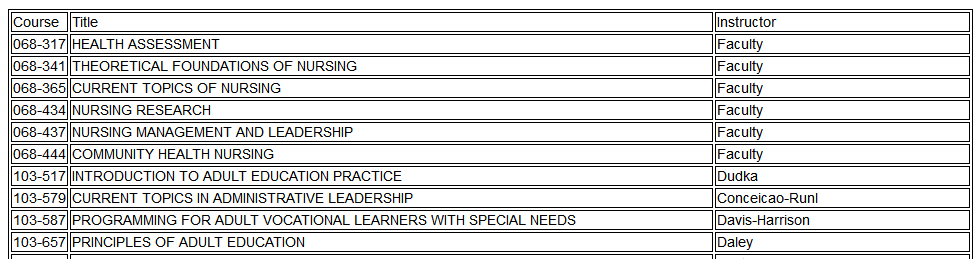
\includegraphics[width=0.95\textwidth]{img/xmloutput.png}
    \caption{Output figure.}
    \label{fig:xmloutput}
\end{figure}
